\section{Merging L1 and L2}

\subsection{New proposal}
\begin{frame}{Burst time and duty-cycle}{}
	\begin{block}{Only 3-9 sec. burst and long break}
		Duty cycle: $T_{Burst}/ T_{Break} \approx 0.3$
	\end{block}

	\begin{figure}[htp]
		\begin{center}
		  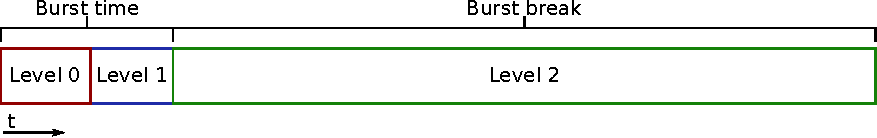
\includegraphics[width=\textwidth]{bursttime}
		  %\caption{Original approach}
		\end{center}
	\end{figure}
	
	\begin{exampleblock}{My proposal to use resources more efficiently}
		Reuse L1 PCs during burst break for L2 computation by combining L1 and L2 to
		one farm
	\end{exampleblock}

	\begin{figure}[htp]
		\begin{center}
		 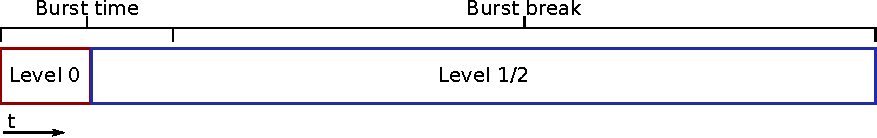
\includegraphics[width=\textwidth]{bursttime-l12merged}
		  %\caption{New proposal}
		\end{center}
	\end{figure}
\end{frame}

\begin{frame}{Don't separate L1 and L2!}{}
	\begin{center} 
		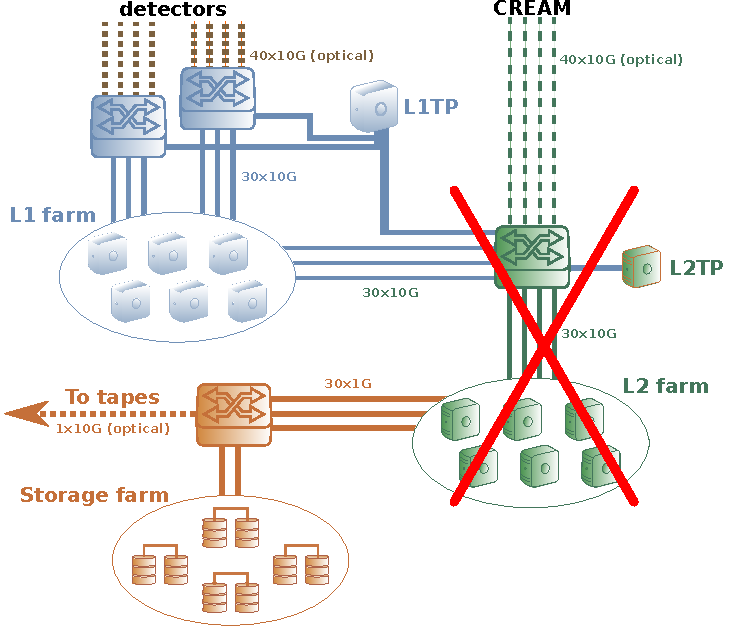
\includegraphics[width=0.8\textwidth]{whole-farm-nol2}
	\end{center} 
\end{frame}

\begin{frame}{Combine L1 and L2 to one farm}{}
	\begin{center} 
		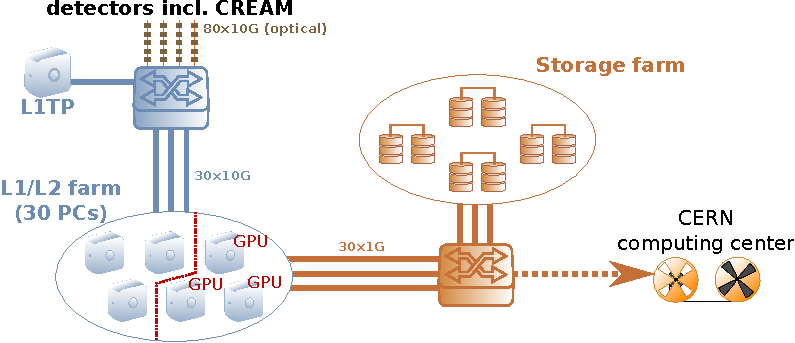
\includegraphics[width=0.9\textwidth]{merged-star}
	\end{center} 
	\begin{exampleblock}{We save about 80k€}
		\begin{itemize}
		  \item No L1 PCs anymore
		  \item Less switches, less network cards
		\end{itemize}
	\end{exampleblock}
\end{frame}


\subsection{Event building @ L1}
\begin{frame}{New proposal}{Event building @ L1}
	\begin{center} 
		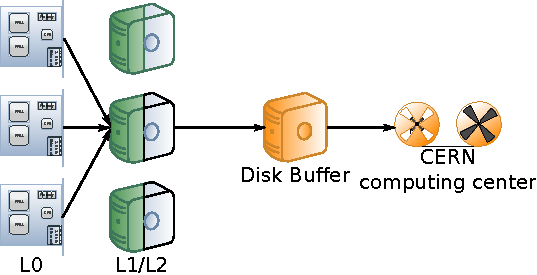
\includegraphics[width=0.6\textwidth]{dataflow-merged-gian}
	\end{center} 
	
	\begin{block}{Every subdetector sends data of an event to one single PC}
		\begin{itemize}
		  	\pro No broadcast of a L1 decision needed anymore (no L1TP)
		  	\pro Easier to implement load balancing (self-sustaining PCs)
  			\contra Every farm PC must serve every subdetector $\Rightarrow$ needs GPUs
		\end{itemize}
	\end{block}
\end{frame}